\section{Processor Optimizations}
\label{sec:processor_opt}

Our processor extensions for exploiting computation and data sparsity in DNN training comprise of frontend and backend extensions in the modern processor pipeline.  The key idea is to optimize existing training loop codes based on speculating that input data will be sparse and executing the optimized loop codes when that happens.  Given the high levels of sparsity in a nunmber of  performance critical portions of DNN training (Figures~\ref{fig:cifar-10_compute_sparsity} and ~\ref{fig:cifar-10_data_sparsity}, most of the execution time is likely to be spent in the optimized loop codes, thus improving training performance greatly. 

\subsection{Back-End Extensions}
Our backend extensions perform two critical functions in the optimization of DNN training code: (i) creating optimized versions of the loops in the training code, and (ii)  enabling the frontend to safely execute the created optimized loop codes for better performance.  Our extensions discover loops to optimize by tracing the stream of committed instructions. The optimized loop codes are kept in a special instruction cache, called the {\it ZOptCache}. We expect the {\it ZOptCache} to be small because there are only a handful (four) kernel loops in DNN training.   We also leverage our cache optimizations described in Section~\ref{sec:cache_opt} to detect when data values are loaded from a zero cacheline. 

\subsubsection{Creating Optimized Loop Codes}
The goal of the optimizer is to generate more efficient versions of training code loops that can boost training performance when executed in place of the original loop codes.  Efficient versions of a loop are created through aggressive loop optimizations based on assumed sparsity in the  loop's data and computation. Multiple optimized code versions could be created for a given loop depending on the different sparsity assumptions.  Thererfore, the execution of optimized loop codes must be predicated on the underlying assumptions being true.  To enable this, the optimizer tags each generated code with description of the conditions that guard its safe execution.  Typical examples of such conditions include the requirement that a particular input data is zero, or that it was loaded from a cacheline containing only zero data values. 

We use the snippet of training code for computing weight deltas in Figure~\ref{fig:deltas_source_code} to illustrate how our optimizer generates efficent versions of training code loops.   A simplified machine code sequence corresponding to  Figure~\ref{fig:deltas_source_code}  is presented in Figure~\ref{fig:deltas_machine_code} as a control flow graph (CFG) of three basic blocks.\footnote{Our example in Figure~\ref{fig:deltas_machine_code} is unoptimized for simplicity of explanation.}  The inner loop of Figure~\ref{fig:deltas_source_code} is represented by the middle block (labelled {\it BB2}), while the outer loop is represented by blocks {\it BB1} and {\it BB3}.  The loop-invariant input, {\it errors[j]}, in Figure~\ref{fig:deltas_source_code} is represented by R1, while the loop-variant inputs, {\it activations[i]} and {\it deltas[k]}, are represented by R3 and R5 respectively. R2 and R7 correspond to the loop counters of the outer and inner loops respectively. 

\begin{figure}[h]
\centering
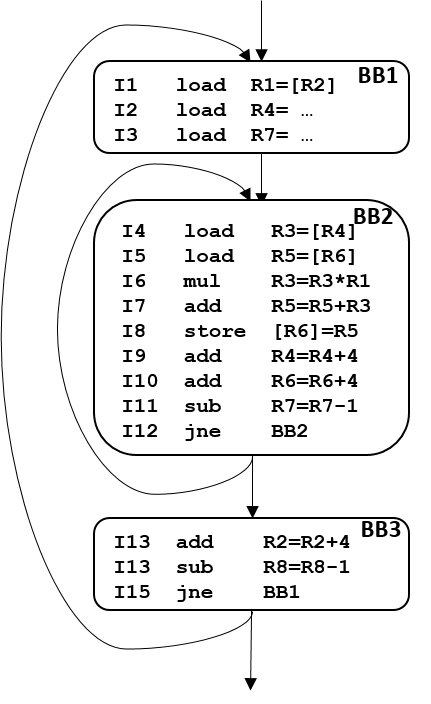
\includegraphics[height=2in]{Figures/weight-delta-code.png}
\caption{Machine code corresponding to the weight deltas computation source code in Figure~\ref{fig:deltas_source_code}.}
\label{fig:deltas_machine_code}
\end{figure}

The key idea of our loop optimizations is to identify input data in the loop, such that if the data was zero it would become possible to safely skip some other instructions or execute those instructions more efficiently.   We refer to the input data that enables optimizations as the {\em anchor} input, and the instructions that can be optimized when the anchor input is zero as zero-optimizable instructions.  For example, if R1 was zero in Figure~\ref{fig:deltas_machine_code}, instruction I$6$ in {\it BB2} could be executed more efficiently (i.e., set to zero), while I$4$, I$5$, I$7$, and I$8$ could all be skipped.  This is because, when R$1$ is zero, R$3$ is set to zero by I$6$ irrespective of the value loaded in I$4$, meaning the I$4$ can be skipped.  Moreover, I$7$ can be skipped because does not change R$5$ since R$3$ is zero, and thus the following store I$8$ will write back the same value loaded from memor by I$5$, meaning that all three instructions can be skipped.  Since all the optimized instructions execute in an inner loop, this optimization is likely to greatly improve performance, and so this simple example demonstrates the effectiveness of that exploiting computation and data sparsity in loops.  As discussed in Section~\ref{subsec:sparse_code_oppor}, a loop can have multiple anchor inputs, each with different performance benefits, and so, for better coverage we create multiple optimized versions of a loop, for different anchor inputs.  

\paragraph{Types of Optimized Loop Codes}
The manner in which an optimized loop code is created depends on static and dynamic properties of the anchor input.  The static property is whether or not the anchor input is loop-invariant, and the dynamic property is whether or not the input is clustered with other input values that are zero (e.g., in a zero cacheline).   Since loop-invariant anchor inputs enable different (and more) optimization opportunities, we create optimized loops of loop-invariant anchor inputs differently than for loop-variant anchor inputs.  However, for good coverage, we construct two optimized loops for each anchor input to handle both cases of when it is a standalone zero value or clustered with other zero data values.   Thus, as discussed below, we create four types of optmized loop codes for: (i)  clustered loop-invariant anchor inputs, (ii) standalone loop-invariant achor inputs, (iii) clustered loop-variant anchor inputs, and (iv) standalone loop-variant anchor inputs.  
 
Figure~\ref{fig:deltas_loop_inv_opt} illustrates how we create optimized loop codes for loop-invariant anchor inputs, using R$1$ in Figure~\ref{fig:deltas_machine_code} as the example anchor input.  Figure~\ref{fig:deltas_loop_inv_opt}(a) shows the optimization for a standalone anchor input, in which execution is steered into an optimized code block ({\it OB1}) after one iteration of {\it BB2}.  This is the optimization example we can studied earlier, in which instructions I$4$---I$8$ could either skipped or executed more efficiently in each iteration of the loop.  Block {\it OB1} executes in place of the remaining iterations of {\it BB2} and ensures that the loop exit invariants are satisfied on entry into {\it BB3}.  Figure~\ref{fig:deltas_loop_inv_opt}(b) shows the optimization for when R$1$ is in a cluster of zero data values, and specifically when R$1$ is the first word in a cacheline of zero data values.  In this case, execution is steered into {\it OB2} which executes in place of the remaining $15$ iterations of {\it BB2} (corresponding to the other R$1$ values in the zero cacheline), before returning control to {\it BB1}.  These two examples show that optimizing for loop-invariant zero data can greatly reduce execution cycles of DNN training loops. 

\begin{figure}[h]
\centering
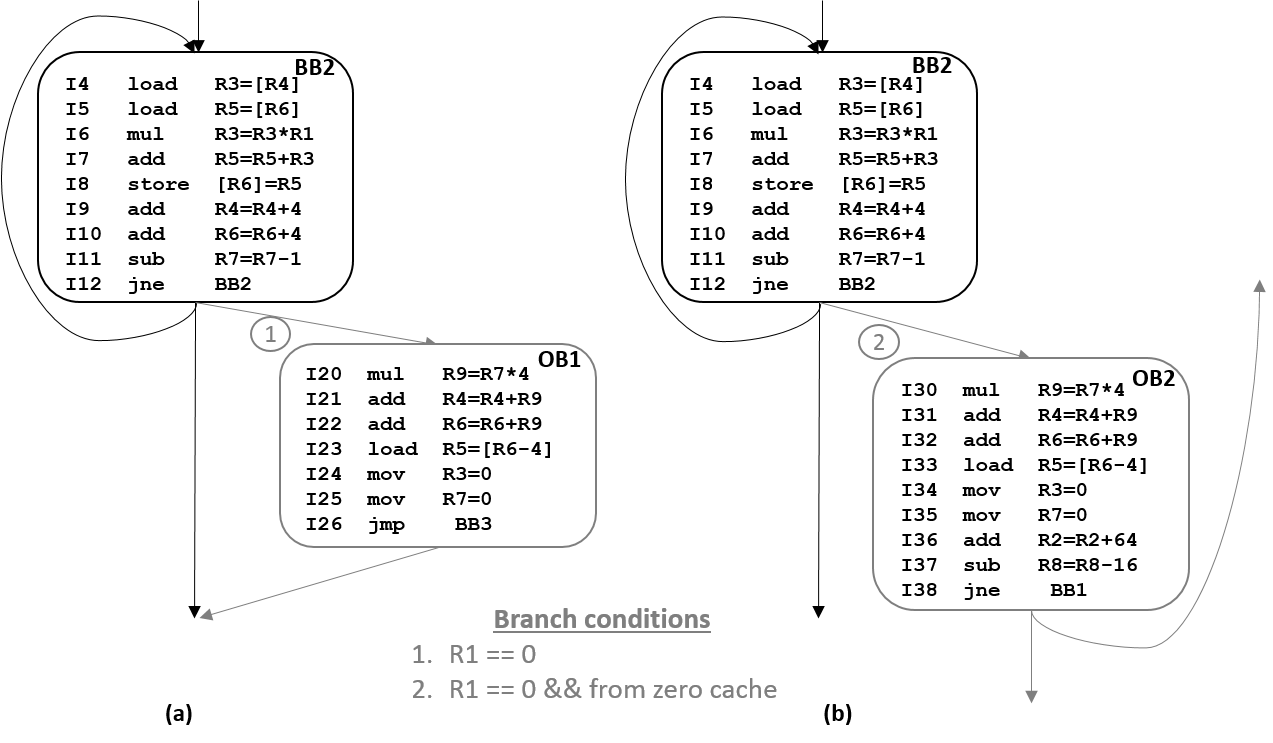
\includegraphics[height=2in, width=.95\columnwidth]{Figures/loop-invariant-zopt.png}
\caption{Optimizing for loop-invariant zero data (R1): (a) for data from data cache, redirect execution to skip inner loop, and (b) for data from zero cache (i.e., cluster of $16$ zero data values) redirect execution to skip 16 executions of inner loop.}
\label{fig:deltas_loop_inv_opt}
\end{figure}

Figure~\ref{fig:deltas_loop_var_opt} illustrates how we create optimized loops for loop-variant anchor inputs, using R$3$ in Figure~\ref{fig:deltas_machine_code} as the example anchor input.  We don't create new code for standalone loop-variant anchor inputs, rather, as shown in Figure~\ref{fig:deltas_loop_var_opt} , we generate code annotations that direct the frontend on how to cheaply optimize the code sequence when the anchor is zero.  In this case, if R$3$ is zero, then in the current iteration I$5$, I$7$, and I$8$ can be skipped, and I$6$ efficiently executed (similar to  if R$1$ is zero).   For the frontend, skipping an instruction simply means squashing it wherever it is in the processor pipeline and making its allocated resources available immediately.   Code annotations are maintained in a special struture called {\it ZOptATable}, which the frontend can quickly access.  Figure~\ref{fig:deltas_loop_var_opt}(b) shows the optimization for when R$3$ is in a cluster of zero data values.  In this case, execution is directed into an optimized block ({\it OB3}) to execute in place of the next ``N'' iterations of {\it BB2}, where ``N'' is minimum of the loop counter R$7$, and the cluster size of zero data values.    

\begin{figure}[h]
\centering
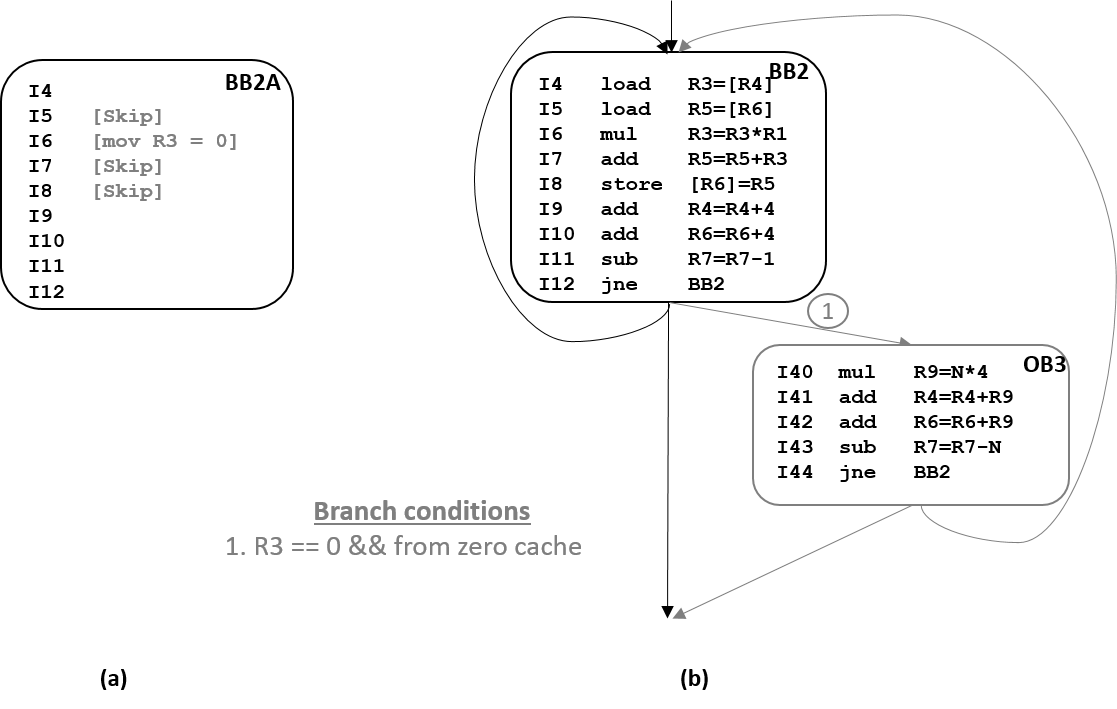
\includegraphics[height=2in, width=.95\columnwidth]{Figures/loop-variant-zopt.png}
\caption{Optimizing for loop-variant zero data (R3):  (a) annotate the code block with actions to be taken by frontend, and (b) redirect execution for data from zero cache.}
\label{fig:deltas_loop_var_opt}
\end{figure}

\subsubsection{Enabling Execution of Optimized Loop Codes}
The primary way that the optimized loop codes get executed is by redirecting the back edge of a loop into the most profitable optimized code that is safe to execute.  This means that at least one iteration of the original loop is always executed before optimized loop codes are executed.  For loops with hundreds (or thousands) of iterations, such as in DNN training workloads, the performance loss is negligible.

  Since instruction fetching takes place in the frontend, the backend maintains a table (a.k.a. {\it ZOptTable}) that maps each loop address in the training code to the set of optimized versions that have being created for it, as well as the conditions under which each optimized version can be executed.   The execution conditions are expressed as invariants on register values as shown in Figures~\ref{fig:deltas_loop_inv_opt} and ~\ref{fig:deltas_loop_var_opt}.  The {\it ZOptTable} also indicates whether the backend has generated code annotations in the {\it ZOptATable} for the frontend to process while executing the optimized code block.  Thus, on a backward jump targetting a loop in the training code, the frontend can efficiently and safely steer execution into optimized code for better performance by checking  the {\it ZOptTable} for optimized versions of the loop and accessing the register files to check for the execution prerequisites.   We expect the {\it ZOptTable} to be relatively small structure (less than $100$ entries) that can be checked quickly to avoid unnnecessary delays on jump instructions.  
    
\subsection{Front-End Extensions}
The frontend extensions of our optimizations are quite minimal to avoid unnecessary critical path delays.  Besides, being responsible for steering executing into optimized loop codes, the frontend also processes code annotations generated by the backend, and tracks data values that loaded from zero cachelines.  The actions requested in the code annotations are easily for the frontend to perform, such as squashing an instruction or setting a register to a constant value (typically zero).   The frontend tracks values that are loaded from zero cachelines through an extra bit the register file.  This bit is set for a destination register if a load request is satified by the zero cahce hierarchy and cleared otherwise.  Also, the bit value is propagated and updated appropriately in the event of register copies and writes. 